\documentclass[12pt,a4paper,oneside]{report}

%% ─── Encodage & langue ────────────────────────────────────────────────────────
\usepackage[T1]{fontenc}
\usepackage[utf8]{inputenc}
\usepackage[french]{babel}
\usepackage{lmodern}
\usepackage{microtype}

%% ─── Mise en page ─────────────────────────────────────────────────────────────
\usepackage{geometry}
\usepackage{setspace}
\usepackage{emptypage}
\geometry{top=2.5cm, bottom=2.5cm, left=3cm, right=2.5cm}
\onehalfspacing

%% ─── Tableaux ─────────────────────────────────────────────────────────────────
\usepackage{array}
\usepackage{longtable}
\usepackage{tabularx}
\usepackage{booktabs}
\usepackage{multirow}

%% ─── Couleurs & graphiques ────────────────────────────────────────────────────
\usepackage{xcolor}
\usepackage{colortbl}
\usepackage{graphicx}
\usepackage{float}
\usepackage{caption}
\captionsetup{labelfont=bf, textfont=it, font=small}

%% ─── Style typographique des titres ───────────────────────────────────────────
\usepackage{titlesec}
\usepackage{titletoc}

%% ─── En-têtes et pieds de page ────────────────────────────────────────────────
\usepackage{fancyhdr}

%% ─── Boîtes colorées ──────────────────────────────────────────────────────────
\usepackage{tcolorbox}
\tcbuselibrary{skins, breakable}

%% ─── Références & bibliographie ───────────────────────────────────────────────
\usepackage[hidelinks]{hyperref}
\usepackage[backend=bibtex, style=numeric, sorting=none]{biblatex}
\addbibresource{references.bib}

%% ═══════════════════════════════════════════════════════════════════════════════
%% PALETTE DE COULEURS
%% ═══════════════════════════════════════════════════════════════════════════════
\definecolor{ustoblue}{RGB}{0,51,102}
\definecolor{ustolightblue}{RGB}{210,228,248}
\definecolor{edugreen}{RGB}{195,235,200}
\definecolor{edudarkgreen}{RGB}{0,100,0}
\definecolor{rowgray}{RGB}{245,245,245}
\definecolor{headerwhite}{RGB}{255,255,255}

%% ═══════════════════════════════════════════════════════════════════════════════
%% STYLE DES CHAPITRES, SECTIONS, SOUS-SECTIONS
%% ═══════════════════════════════════════════════════════════════════════════════
\titleformat{\chapter}[block]
  {\normalfont\LARGE\bfseries\color{ustoblue}}
  {Chapitre~\thechapter~\textemdash~}{0pt}{\LARGE\bfseries}
\titlespacing*{\chapter}{0pt}{0pt}{28pt}

\titleformat{\section}
  {\normalfont\large\bfseries\color{ustoblue}}
  {\thesection}{1em}{}
\titlespacing*{\section}{0pt}{14pt}{6pt}

\titleformat{\subsection}
  {\normalfont\normalsize\bfseries\color{black}}
  {\thesubsection}{1em}{}
\titlespacing*{\subsection}{0pt}{10pt}{4pt}

\titleformat{\paragraph}[runin]
  {\normalfont\normalsize\bfseries}
  {}{0pt}{}[~\textemdash~]

%% ═══════════════════════════════════════════════════════════════════════════════
%% EN-TÊTES ET PIEDS DE PAGE
%% ═══════════════════════════════════════════════════════════════════════════════
\pagestyle{fancy}
\fancyhf{}
\fancyhead[L]{\parbox[c]{0.44\headwidth}{\small\itshape USTO-MB~---~D\'ep. Informatique}}
\fancyhead[R]{\parbox[c]{0.44\headwidth}{\small\itshape\raggedleft\nouppercase{\leftmark}}}
\fancyfoot[C]{\small ---~\thepage~---}
\renewcommand{\headrulewidth}{0.5pt}
\renewcommand{\footrulewidth}{0.3pt}

% Style pour pages spéciales (TOC, LOF, LOT)
\fancypagestyle{plain}{%
  \fancyhf{}%
  \fancyfoot[C]{\small ---~\thepage~---}%
  \renewcommand{\headrulewidth}{0pt}%
}

%% ═══════════════════════════════════════════════════════════════════════════════
%% BOÎTE D'INSTRUCTIONS FIGURE (à supprimer avant soumission finale)
%% ═══════════════════════════════════════════════════════════════════════════════
\newtcolorbox{figurebox}[1]{
  colback  = ustolightblue!35,
  colframe = ustoblue,
  coltitle = white,
  fonttitle= \bfseries\small,
  title    = {Instruction figure~---~#1},
  breakable,
  left=6pt, right=6pt, top=4pt, bottom=4pt,
  before=\medskip, after=\medskip,
  sharp corners=south
}

%% ═══════════════════════════════════════════════════════════════════════════════
%% COMMANDE IMAGE SÉCURISÉE (placeholder si fichier absent)
%% ═══════════════════════════════════════════════════════════════════════════════
\newcommand{\safeimage}[4][0.85\textwidth]{%
  \begin{figure}[H]
    \centering
    \IfFileExists{#2}{%
      \includegraphics[width=#1]{#2}%
    }{%
      \fcolorbox{ustoblue}{ustolightblue!20}{%
        \parbox[c][3.5cm][c]{0.88\textwidth}{\centering
          \color{ustoblue}\textbf{[Emplacement r\'eserv\'e~---~Figure~#3]}\\[6pt]
          \small Fichier attendu~:~\texttt{#2}\\[4pt]
          \textit{\color{gray}Remplacer par l'image avant soumission}
        }%
      }%
    }%
    \caption{#4}
    \label{fig:#3}
  \end{figure}%
}

%% ═══════════════════════════════════════════════════════════════════════════════
%% DOCUMENT
%% ═══════════════════════════════════════════════════════════════════════════════
\begin{document}

\pagenumbering{roman}
\tableofcontents
\clearpage
\listoffigures
\clearpage
\listoftables
\clearpage

\pagenumbering{arabic}
\setcounter{page}{1}

%% ═══════════════════════════════════════════════════════════════════════════════
%% INTRODUCTION GENERALE
%% ═══════════════════════════════════════════════════════════════════════════════

\chapter*{Introduction generale}
\addcontentsline{toc}{chapter}{Introduction generale}

La transformation numerique des systemes d'enseignement superieur constitue aujourd'hui une priorite strategique pour les etablissements confrontes a la massification des effectifs, a la diversification des parcours et a l'exigence croissante de qualite pedagogique. Dans ce contexte, la mise en place de plateformes numeriques ne peut plus se limiter a la simple diffusion de supports de cours: elle doit integrer la gouvernance academique, la collaboration entre acteurs et la traçabilite des activites.

Le projet \textbf{EduConnect} s'inscrit dans cette dynamique. Il vise a proposer une plateforme unifiee de partage pedagogique et de collaboration, adaptee au contexte universitaire local, en combinant: gestion par roles, structuration des ressources par niveau/module/composant, communication synchrone et asynchrone, et outils de pilotage administratifs.

Sur le plan methodologique, ce memoire est construit en coherence avec les pratiques observees dans les memoires de reference du meme encadrement (application de branding et bibliotheque virtuelle), tout en les etendant a une architecture SaaS educative multi-ecole et a une logique startup.

\paragraph{Problematique generale.}
Comment concevoir une plateforme academique a la fois robuste techniquement, pertinente pedagogiquement et viable economiquement, capable d'unifier les usages quotidiens des etudiants, formateurs et administrations?

\paragraph{Objectif global.}
Concevoir, implementer et evaluer EduConnect comme solution complete, puis en proposer un cadre de passage a l'echelle startup a travers un modele economique et une strategie de croissance.

\paragraph{Organisation du memoire.}
Ce memoire est structure en quatre chapitres:
\begin{itemize}
  \item \textbf{Chapitre 1}: Contexte, problematique et etat de l'art;
  \item \textbf{Chapitre 2}: Analyse des besoins, modelisation UML et conception;
  \item \textbf{Chapitre 3}: Realisation technique, deploiement et validation;
  \item \textbf{Chapitre 4}: Modele economique startup, SWOT et feuille de route.
\end{itemize}

L'enchainement de ces chapitres permet de relier de maniere progressive la pertinence scientifique du projet, sa realisation concrete et sa projection entrepreneuriale.

%% ═══════════════════════════════════════════════════════════════════════════════
%% CHAPITRE 1 — Contexte général, problématique et état de l'art
%% ═══════════════════════════════════════════════════════════════════════════════

\chapter{Contexte g\'en\'eral, probl\'ematique et \'etat de l'art}

%%──────────────────────────────────────────────────────────────────────────────
\section{Introduction du chapitre}
%%──────────────────────────────────────────────────────────────────────────────

La g\'en\'eralisation des technologies num\'eriques dans l'enseignement sup\'erieur constitue aujourd'hui l'un des leviers strat\'egiques les plus significatifs pour l'am\'elioration de la qualit\'e p\'edagogique, la continuit\'e des activit\'es acad\'emiques et l'inclusion \'educative. Dans ce contexte de mutation profonde, les \'etablissements universitaires sont confront\'es \`a un imp\'eratif d'adaptation organisationnelle et technologique, auquel r\'epondent des environnements num\'eriques de plus en plus sophistiqu\'es~\cite{unesco_digital_2026,worldbank_edtech_2026}.

Le pr\'esent chapitre constitue le socle analytique et conceptuel du projet \textbf{EduConnect}. Il poursuit quatre objectifs compl\'ementaires~: (i)~d\'ecrire le contexte mondial et national de la transformation num\'erique de l'enseignement~; (ii)~formuler la probl\'ematique ayant motiv\'e la conception d'EduConnect~; (iii)~pr\'esenter les objectifs et la m\'ethodologie adopt\'es~; et (iv)~dresser un \'etat de l'art approfondi des solutions existantes, afin de positionner EduConnect par rapport aux r\'ef\'erences du domaine.

Ce chapitre est organis\'e comme suit~: la section~\ref{sec:contexte} traite du contexte g\'en\'eral~; la section~\ref{sec:problematique} formule la probl\'ematique~; la section~\ref{sec:objectifs} d\'etaille les objectifs~; la section~\ref{sec:methodo} pr\'esente la d\'emarche m\'ethodologique~; la section~\ref{sec:etat_art} constitue l'\'etat de l'art~; la section~\ref{sec:positionnement} positionne EduConnect~; la section~\ref{sec:figures} pr\'esente les figures requises~; enfin, la section~\ref{sec:conclusion} conclut le chapitre.

%%──────────────────────────────────────────────────────────────────────────────
\section{Contexte g\'en\'eral}
\label{sec:contexte}
%%──────────────────────────────────────────────────────────────────────────────

\subsection{Transformation num\'erique de l'enseignement sup\'erieur \`a l'\'echelle mondiale}

La transformation num\'erique de l'\'education s'est acc\'el\'er\'ee de mani\`ere consid\'erable au cours de la derni\`ere d\'ecennie, port\'ee par la g\'en\'eralisation de l'acc\`es \`a Internet, la mont\'ee en puissance des technologies mobiles et, plus r\'ecemment, l'\'emergence de l'intelligence artificielle appliqu\'ee aux processus p\'edagogiques. L'Union internationale des t\'el\'ecommunications (UIT) indique que 6~milliards de personnes, soit environ 74\,\% de la population mondiale, utilisaient Internet en 2025, tout en soulignant que 2,2~milliards d'individus demeurent exclus de cet acc\`es, principalement dans les pays \`a revenus faibles et interm\'ediaires~\cite{itu_facts_2025}.

L'UNESCO confirme que si la connectivit\'e progresse \`a l'\'echelle mondiale, elle reste profond\'ement in\'egale~: seulement 40\,\% des \'ecoles primaires et 50\,\% des \'etablissements du secondaire inf\'erieur sont connect\'es \`a Internet dans le monde~\cite{unesco_gem_2023}. Ces donn\'ees soul\`event des questions fondamentales de politique \'educative et d'\'equit\'e d'acc\`es aux ressources num\'eriques, que l'UNESCO aborde dans ses cadres de comp\'etences num\'eriques et ses recommandations sur les ressources \'educatives libres~\cite{unesco_oer_2019,unesco_digital_2026}.

La Banque mondiale souligne que l'EdTech repr\'esente une opportunit\'e in\'edite pour les pays \`a revenus interm\'ediaires~: si elle est soutenue par des comp\'etences num\'eriques fondamentales et une connectivit\'e ad\'equate, elle peut contribuer \`a r\'eduire la crise d'apprentissage mondiale, notamment dans les communaut\'es souffrant de p\'enurie d'enseignants~\cite{worldbank_edtech_2026}. Toutefois, cette m\^eme institution met en garde contre les risques li\'es \`a la s\'ecurit\'e des donn\'ees et le risque d'aggravation des in\'egalit\'es \'educatives en l'absence de politiques d'encadrement adapt\'ees.

\subsection{Contexte national et enjeux institutionnels}

Dans le contexte alg\'erien et plus particuli\`erement au sein des universit\'es telles que l'Universit\'e des Sciences et de la Technologie d'Oran Mohamed~Boudiaf (USTO-MB), la gestion des activit\'es p\'edagogiques souffre d'une fragmentation des outils et des canaux de diffusion. Les ressources sont souvent partag\'ees via des messageries instantan\'ees non structur\'ees, les annonces ne parviennent pas syst\'ematiquement aux \'etudiants concern\'es, et les enseignants manquent d'un espace centralis\'e pour organiser leurs productions p\'edagogiques par module et par niveau d'\'etudes.

Ce constat est confirme par les deux travaux de reference utilises dans votre encadrement: le memoire sur la bibliotheque virtuelle de partage de livres~\cite{memoire_bibliotheque_2025}, qui met en avant la diffusion structuree des ressources, et le memoire sur l'application mobile de branding~\cite{memoire_branding_2025}, qui insiste sur l'architecture orientee utilisateur et la qualite de l'experience. Le present memoire reprend volontairement cette logique de redaction (contexte, conception, implementation, evaluation), tout en l'etendant a un cadre SaaS educatif multi-ecole et a une projection startup.

%%──────────────────────────────────────────────────────────────────────────────
\section{Probl\'ematique}
\label{sec:problematique}
%%──────────────────────────────────────────────────────────────────────────────

La gestion des activit\'es p\'edagogiques dans un contexte universitaire contemporain fait face \`a un d\'efi central~: la multiplicit\'e des outils et des canaux de communication g\'en\`ere une dispersion informationnelle qui nuit \`a la coh\'erence de l'exp\'erience acad\'emique. Les ressources p\'edagogiques~--- cours, travaux dirig\'es, travaux pratiques, examens, corrig\'es et supports multim\'edias~--- sont dispers\'ees sur des supports h\'et\'erog\`enes, sans structuration par module ni tra\c{c}abilit\'e des mises \`a jour.

Par ailleurs, la communication entre enseignants, mod\'erateurs et \'etudiants s'appuie souvent sur des outils grand public non con\c{c}us pour les usages acad\'emiques, ce qui engendre des probl\`emes de s\'ecurit\'e, de gouvernance et de qualit\'e de service. L'absence d'un syst\`eme de notification centralis\'e, d'un espace de publication structur\'e et d'un planificateur int\'egr\'e contraint les acteurs \`a recourir \`a des solutions de contournement chronophages et peu fiables.

\medskip
\noindent\fcolorbox{ustoblue}{ustolightblue!20}{\parbox{0.96\textwidth}{%
\textbf{Question de recherche~:} Comment concevoir et d\'evelopper une plateforme num\'erique unifi\'ee, s\'ecuris\'ee et modulaire, capable de centraliser les ressources p\'edagogiques, de faciliter la communication entre les diff\'erents acteurs de la communaut\'e acad\'emique, et de soutenir l'organisation du travail collectif, tout en restant accessible, maintenable et adapt\'ee au contexte universitaire local\,?
}}
\medskip

%%──────────────────────────────────────────────────────────────────────────────
\section{Objectifs du projet}
\label{sec:objectifs}
%%──────────────────────────────────────────────────────────────────────────────

\subsection{Objectif g\'en\'eral}

L'objectif g\'en\'eral du projet est de concevoir, d\'evelopper et valider \textbf{EduConnect}~: une plateforme web de partage p\'edagogique et de collaboration acad\'emique, con\c{c}ue pour les usages universitaires et structur\'ee autour d'une architecture orient\'ee modules, d'un syst\`eme de gouvernance par r\^oles et d'une couche sociale int\'egr\'ee.

\subsection{Objectifs sp\'ecifiques}

\begin{itemize}
  \item[\textbf{OS1.}] Centraliser les ressources p\'edagogiques (cours, TD, TP, examens, corrig\'es, playlists) dans une architecture hi\'erarchique~: Niveau $\rightarrow$ Module $\rightarrow$ Section $\rightarrow$ Ressource.
  \item[\textbf{OS2.}] Mettre en \oe uvre un syst\`eme d'authentification s\'ecuris\'e par jetons JWT et une autorisation par r\^oles~: Administrateur global, Mod\'erateur et Utilisateur.
  \item[\textbf{OS3.}] Int\'egrer un espace de communication structur\'e~: publications, commentaires, votes, partages et messagerie instantan\'ee (chat priv\'e et de groupe).
  \item[\textbf{OS4.}] D\'evelopper un syst\`eme de notifications permettant le suivi des \'ev\'enements acad\'emiques avec compteur de non-lus.
  \item[\textbf{OS5.}] Proposer un planificateur hebdomadaire pour la gestion collective des activit\'es et des \'ech\'eances.
  \item[\textbf{OS6.}] Garantir la tra\c{c}abilit\'e compl\`ete des actions de gestion~: ajout, modification et suppression des ressources, contr\^ol\'ees par le syst\`eme de r\^oles.
\end{itemize}

%%──────────────────────────────────────────────────────────────────────────────
\section{D\'emarche m\'ethodologique}
\label{sec:methodo}
%%──────────────────────────────────────────────────────────────────────────────

La d\'emarche adopt\'ee suit un processus incr\'emental en cinq phases, conforme aux pratiques reconnues en ing\'enierie des syst\`emes d'information et aux recommandations des travaux de r\'ef\'erence analys\'es~:

\begin{enumerate}
  \item \textbf{Analyse des besoins}~: identification des besoins fonctionnels et non fonctionnels par l'\'etude des usages existants, l'analyse de la litt\'erature et la consultation des trois m\'emoires de r\'ef\'erence.
  \item \textbf{Mod\'elisation conceptuelle}~: repr\'esentation des interactions par des diagrammes UML (cas d'utilisation, s\'equence, classes) pour formaliser les sc\'enarios et l'architecture logique.
  \item \textbf{Conception de l'architecture}~: d\'efinition de l'architecture applicative (API REST, frontend SPA) et du sch\'ema de la base de donn\'ees relationnelle PostgreSQL.
  \item \textbf{Impl\'ementation et int\'egration}~: d\'eveloppement progressif par fonctionnalit\'es (authentification, ressources, social, notifications, planificateur, administration), avec validation continue.
  \item \textbf{Tests et ajustements}~: validation fonctionnelle, tests de s\'ecurit\'e et ajustements selon les retours d'exp\'erience.
\end{enumerate}

%%──────────────────────────────────────────────────────────────────────────────
\section{\'Etat de l'art}
\label{sec:etat_art}
%%──────────────────────────────────────────────────────────────────────────────

\subsection{D\'efinitions et concepts cl\'es}

\paragraph{Syst\`eme de gestion de l'apprentissage (LMS).}
Un LMS (\textit{Learning Management System}) est un logiciel permettant de cr\'eer, distribuer et g\'erer du contenu p\'edagogique, ainsi que de suivre la progression des apprenants~\cite{moodle_overview_2026}. Les principaux LMS du march\'e incluent Moodle, Canvas et Blackboard.

\paragraph{Plateforme collaborative.}
Une plateforme collaborative est un environnement num\'erique qui offre des fonctionnalit\'es de communication, de co-production et de gestion des activit\'es pour des groupes d'utilisateurs. Elle peut int\'egrer des outils de messagerie, de partage de fichiers, de planification et de gestion de projets.

\paragraph{Apprentissage en ligne (\textit{e-learning}).}
L'e-learning d\'esigne l'ensemble des modalit\'es d'enseignement et d'apprentissage faisant appel aux technologies num\'eriques, qu'elles soient synchrones (classes virtuelles, visioconf\'erence) ou asynchrones (cours en ligne, forums, documents partag\'es)~\cite{unesco_digital_2026}.

\subsection{Pr\'esentation des solutions de r\'ef\'erence}

\paragraph{Moodle.}
Moodle est l'un des LMS open source les plus utilis\'es dans le monde. Il offre une gestion fine des cours, des activit\'es et des \'evaluations, ainsi qu'un syst\`eme d'extensions (plugins) permettant une forte personnalisation. Sa gouvernance institutionnelle est tr\`es flexible, mais son d\'eploiement exige des comp\'etences techniques~\cite{moodle_overview_2026}.

\paragraph{Google Classroom.}
Google Classroom est un service cloud de gestion de classes orient\'e simplicit\'e. Il s'int\`egre nativement aux outils Google Workspace (Drive, Docs, Meet). Sa personnalisation reste cependant limit\'ee et sa d\'ependance \`a l'\'ecosyst\`eme propri\'etaire peut constituer une contrainte~\cite{google_classroom_2026}.

\paragraph{Microsoft Teams pour l'\'Education.}
Microsoft Teams Education offre une exp\'erience unifi\'ee de classe virtuelle et de collaboration au sein de l'environnement Microsoft~365. Il supporte la visioconf\'erence, le chat, la gestion d'\'equipes et les devoirs~\cite{microsoft_teams_edu_2026}.

\paragraph{Canvas LMS.}
Canvas est un LMS cloud moderne, appr\'eci\'e pour son interface structur\'ee, ses workflows d'\'evaluation et ses outils analytiques. Son adoption est pr\'edominante dans les universit\'es nord-am\'ericaines~\cite{canvas_overview_2026}.

%%──────────────────────────────────────────────────────────────────────────────
\subsection{Tableau~1~---~Comparaison synth\'etique des plateformes}
%%──────────────────────────────────────────────────────────────────────────────

Le tableau~\ref{tab:compar_synth} offre une vue d'ensemble des quatre plateformes de r\'ef\'erence selon quatre axes strat\'egiques~: positionnement, points forts, limites et pertinence dans le contexte local de l'USTO-MB.

\renewcommand{\arraystretch}{1.8}
{\setlength{\tabcolsep}{7pt}
\begin{table}[H]
\centering
\caption{Tableau synth\'etique des plateformes p\'edagogiques num\'eriques (vue d'ensemble)}
\label{tab:compar_synth}
\begin{tabular}{|>{\bfseries}p{2.3cm}|p{2.5cm}|p{3.2cm}|p{3.0cm}|p{2.2cm}|}

%% ── EN-TÊTE ────────────────────────────────────────────────────────────
\hline
\rowcolor{ustoblue}
\textcolor{white}{\textbf{Plateforme}} &
\textcolor{white}{\textbf{Positionnement}} &
\textcolor{white}{\textbf{Points forts}} &
\textcolor{white}{\textbf{Limites}} &
\textcolor{white}{\textbf{Pertinence locale}} \\
\hline

%% ── LIGNE 1 ────────────────────────────────────────────────────────────
\rowcolor{ustolightblue!40}
Moodle &
LMS open source &
Flexibilit\'e, plugins, structure p\'edagogique fine &
Maintenance technique exigeante &
\'Elev\'ee (mais complexe) \\
\hline

%% ── LIGNE 2 ────────────────────────────────────────────────────────────
\rowcolor{rowgray}
Google Classroom &
Classe et devoirs cloud &
Simplicit\'e, int\'egration Google Workspace &
D\'ependance Google, personnalisation limit\'ee &
Moyenne \\
\hline

%% ── LIGNE 3 ────────────────────────────────────────────────────────────
\rowcolor{ustolightblue!40}
MS Teams Edu &
Collaboration + classe &
Communication unifi\'ee, visioconf\'erence &
Complexit\'e pour usages purement p\'edagogiques &
Moyenne \\
\hline

%% ── LIGNE 4 ────────────────────────────────────────────────────────────
\rowcolor{rowgray}
Canvas LMS &
LMS cloud moderne &
Interface structur\'ee, analytics &
Co\^ut selon contexte institutionnel &
Faible \`a moyenne \\
\hline

\end{tabular}
\end{table}}

\noindent{\small\textit{Sources~:~\cite{moodle_overview_2026,google_classroom_2026,microsoft_teams_edu_2026,canvas_overview_2026}}}

%%──────────────────────────────────────────────────────────────────────────────
%% BLOC DE TRANSITION ENTRE LES DEUX TABLEAUX
%%──────────────────────────────────────────────────────────────────────────────

\medskip
\begin{tcolorbox}[
  colback  = ustolightblue!20,
  colframe = ustoblue,
  coltitle = white,
  fonttitle= \bfseries,
  title    = {Observations cl\'es issues du tableau~\ref{tab:compar_synth}~---~vers une analyse crit\`ere par crit\`ere},
  left=8pt, right=8pt, top=6pt, bottom=6pt,
  sharp corners=south
]
\begin{itemize}
  \item Aucune des quatre solutions g\'en\'eralistes n'est con\c{c}ue sp\'ecifiquement pour le contexte universitaire alg\'erien~; leur adaptation exige des ressources techniques et financi\`eres importantes.
  \item EduConnect est la seule solution \textbf{gratuite}, \textbf{auto-h\'eberg\'ee} et \textbf{contexte-native}~: chaque fonctionnalit\'e a \'et\'e con\c{c}ue en r\'eponse directe \`a un besoin identifi\'e \`a l'USTO-MB.
  \item Le tableau~\ref{tab:compar_detail} ci-dessous approfondit l'analyse sur \textbf{12 crit\`eres fonctionnels et techniques}, permettant de mesurer pr\'ecis\'ement les apports sp\'ecifiques d'EduConnect.
\end{itemize}
\end{tcolorbox}
\medskip

%%──────────────────────────────────────────────────────────────────────────────
\subsection{Tableau~2~---~Analyse comparative d\'etaill\'ee (12 crit\`eres)}
%%──────────────────────────────────────────────────────────────────────────────

Le tableau~\ref{tab:compar_detail} confronte les quatre plateformes de r\'ef\'erence sur douze crit\`eres couvrant les dimensions fonctionnelles, techniques, organisationnelles et \'economiques.

\renewcommand{\arraystretch}{1.8}
\setlength{\tabcolsep}{7pt}
\begin{longtable}{|>{\bfseries\raggedright\arraybackslash}p{3.5cm}|
                   >{\raggedright\arraybackslash}p{2.5cm}|
                   >{\raggedright\arraybackslash}p{2.5cm}|
                   >{\raggedright\arraybackslash}p{2.5cm}|
                   >{\raggedright\arraybackslash}p{2.5cm}|}

\caption{Analyse comparative d\'etaill\'ee des plateformes p\'edagogiques num\'eriques (12 crit\`eres)}
\label{tab:compar_detail} \\

%% ── EN-TÊTE PREMIÈRE PAGE ──────────────────────────────────────────────
\hline
\rowcolor{ustoblue}
\textcolor{white}{\textbf{Crit\`ere}} &
\textcolor{white}{\textbf{Moodle}} &
\textcolor{white}{\textbf{G. Classroom}} &
\textcolor{white}{\textbf{MS Teams}} &
\textcolor{white}{\textbf{Canvas}} \\
\hline
\endfirsthead

%% ── EN-TÊTE PAGES SUIVANTES ────────────────────────────────────────────
\multicolumn{5}{l}{\small\textit{(suite du tableau~\ref{tab:compar_detail})}} \\[2pt]
\hline
\rowcolor{ustoblue}
\textcolor{white}{\textbf{Crit\`ere}} &
\textcolor{white}{\textbf{Moodle}} &
\textcolor{white}{\textbf{G. Classroom}} &
\textcolor{white}{\textbf{MS Teams}} &
\textcolor{white}{\textbf{Canvas}} \\
\hline
\endhead

\hline
\multicolumn{5}{r|}{\small\textit{Suite page suivante\ldots}} \\
\endfoot

\hline
\endlastfoot

%% ── CRITÈRE 1 ──────────────────────────────────────────────────────────
\rowcolor{ustolightblue!40}
Mode de d\'eploiement &
Auto-h\'eberg\'e\,/ cloud &
Cloud Google &
Cloud Microsoft &
Cloud \\
\hline

%% ── CRITÈRE 2 ──────────────────────────────────────────────────────────
\rowcolor{rowgray}
Orientation principale &
LMS complet &
Classe et devoirs &
Collaboration + classe &
LMS complet \\
\hline

%% ── CRITÈRE 3 ──────────────────────────────────────────────────────────
\rowcolor{ustolightblue!40}
Gestion des ressources &
Avanc\'ee (cours, banques) &
Essentielle (devoirs) &
Correcte (canaux) &
Avanc\'ee \\
\hline

%% ── CRITÈRE 4 ──────────────────────────────────────────────────────────
\rowcolor{rowgray}
Organisation par modules &
Partielle (cat\'eg.) &
Par classe uniquement &
Par \'equipe\,/\,canal &
Par cours \\
\hline

%% ── CRITÈRE 5 ──────────────────────────────────────────────────────────
\rowcolor{ustolightblue!40}
Syst\`eme de r\^oles &
Oui (multiples) &
Enseignant\,/\,\'El\`eve &
Propri\'etaire\,/\,Membre &
Admin\,/\,\'Etudiant \\
\hline

%% ── CRITÈRE 6 ──────────────────────────────────────────────────────────
\rowcolor{rowgray}
Publications et commentaires &
Forums de discussion &
Commentaires de flux &
Canaux de discussion &
Annonces de cours \\
\hline

%% ── CRITÈRE 7 ──────────────────────────────────────────────────────────
\rowcolor{ustolightblue!40}
Chat int\'egr\'e &
Via plugin &
Non (externe) &
Oui (complet) &
Partiel \\
\hline

%% ── CRITÈRE 8 ──────────────────────────────────────────────────────────
\rowcolor{rowgray}
Notifications &
Courriel\,/\,interne &
Courriel Google &
Notifications M365 &
Courriel\,/\,interne \\
\hline

%% ── CRITÈRE 9 ──────────────────────────────────────────────────────────
\rowcolor{ustolightblue!40}
Planificateur &
Agenda basique &
Google Agenda (ext.) &
Calendrier M365 &
Calendrier int\'egr\'e \\
\hline

%% ── CRITÈRE 10 ─────────────────────────────────────────────────────────
\rowcolor{rowgray}
Technologies &
PHP, MySQL &
Cloud Google &
Cloud Microsoft &
Ruby, PostgreSQL \\
\hline

%% ── CRITÈRE 11 ─────────────────────────────────────────────────────────
\rowcolor{ustolightblue!40}
Co\^ut\,/\,Licence &
Gratuit (open source) &
Gratuit (Google) &
Payant (M365) &
Payant (licence) \\
\hline

%% ── CRITÈRE 12 ─────────────────────────────────────────────────────────
\rowcolor{rowgray}
Adaptation locale &
\'Elev\'ee avec configuration &
Moyenne &
Moyenne &
Faible \\
\hline

\end{longtable}

\noindent{\small\textit{Sources~: \cite{moodle_overview_2026,google_classroom_2026,microsoft_teams_edu_2026,canvas_overview_2026}}}

\subsection{Synth\`ese et bilan de l'\'etat de l'art}

L'analyse comparative men\'ee dans les tableaux~\ref{tab:compar_synth} et~\ref{tab:compar_detail} confirme que les plateformes g\'en\'eralistes existantes couvrent partiellement les besoins identifi\'es dans notre contexte~: Moodle excelle dans la gestion p\'edagogique mais exige une expertise technique importante~; Google Classroom privil\'egie la simplicit\'e au d\'etriment de la personnalisation~; Microsoft Teams est optimis\'e pour la collaboration mais reste secondaire en mati\`ere d'organisation p\'edagogique fine~; enfin, Canvas est trop co\^uteux et peu adapt\'e aux contraintes institutionnelles locales.

Ces lacunes cumul\'ees justifient la conception d'EduConnect~: une solution \'elabor\'ee sp\'ecifiquement pour le contexte acad\'emique local, gratuite, auto-h\'eberg\'ee, et combinant dans un seul environnement la gestion modulaire des ressources, la gouvernance par r\^oles, la communication int\'egr\'ee et la planification hebdomadaire.

%%──────────────────────────────────────────────────────────────────────────────
\section{Positionnement d'EduConnect}
\label{sec:positionnement}
%%──────────────────────────────────────────────────────────────────────────────

EduConnect se positionne comme une plateforme acad\'emique int\'egr\'ee, r\'eunissant dans un seul environnement les fonctions p\'edagogiques, sociales et organisationnelles que les solutions existantes dispersent entre plusieurs outils. Son architecture repose sur quatre piliers structurants~:

\begin{itemize}
  \item \textbf{Navigation module-first~:} la granularit\'e p\'edagogique est au c\oe ur de l'exp\'erience~; chaque module dispose d'une page d\'edi\'ee regroupant ses sections et ses ressources class\'ees par type.
  \item \textbf{Gouvernance par r\^oles~:} le syst\`eme d'autorisation \`a trois niveaux (Administrateur global, Mod\'erateur, Utilisateur) garantit la s\'ecurit\'e, la modulation des acc\`es et la responsabilit\'e de chaque acteur.
  \item \textbf{Couche sociale et collaborative~:} les publications, le chat et les notifications constituent un tissu de communication acad\'emique structur\'e, tra\c{c}able et centralis\'e.
  \item \textbf{Dimension op\'erationnelle~:} le planificateur hebdomadaire transforme EduConnect en outil de gestion du travail acad\'emique, au-del\`a du simple partage de ressources.
\end{itemize}

%%──────────────────────────────────────────────────────────────────────────────
\section{Illustrations de la plateforme EduConnect}
\label{sec:figures}
%%──────────────────────────────────────────────────────────────────────────────

Cette section pr\'esente les captures d'\'ecran de la plateforme illustrant les fonctionnalit\'es d\'ecrites dans les sections pr\'ec\'edentes.

%%──────────────────────────
\subsection{Figure~1~---~Capture~: navigation par modules}

\begin{figurebox}{Figure~1~---~Capture d'écran à prendre}
\textbf{Ce que vous devez capturer~:} L'interface principale montrant les modules p\'edagogiques.

\textbf{Proc\'edure~:}
\begin{enumerate}
  \item Ouvrir un terminal dans le dossier \texttt{site\_partage/backend/} et ex\'ecuter~: \texttt{node server.js}
  \item Ouvrir \texttt{index.html} dans le navigateur, se connecter~: matricule \textbf{admin-2026}, mot de passe \textbf{Admin@2026}.
  \item Naviguer vers la page d'accueil affichant les modules (Licence\,/\,Master\,/\,Doctorat).
  \item Passer en plein \'ecran (F11), capturer avec \textbf{Win\,+\,Shift\,+\,S}, coller dans Paint, enregistrer.
  \item Enregistrer sous~: \texttt{figures/F1\_interface\_modules.png}
\end{enumerate}
\textbf{Objectif~:} Montrer la navigation orient\'ee modules qui diff\'erencie EduConnect des LMS classiques.
\end{figurebox}

\begin{figure}[H]
  \centering
  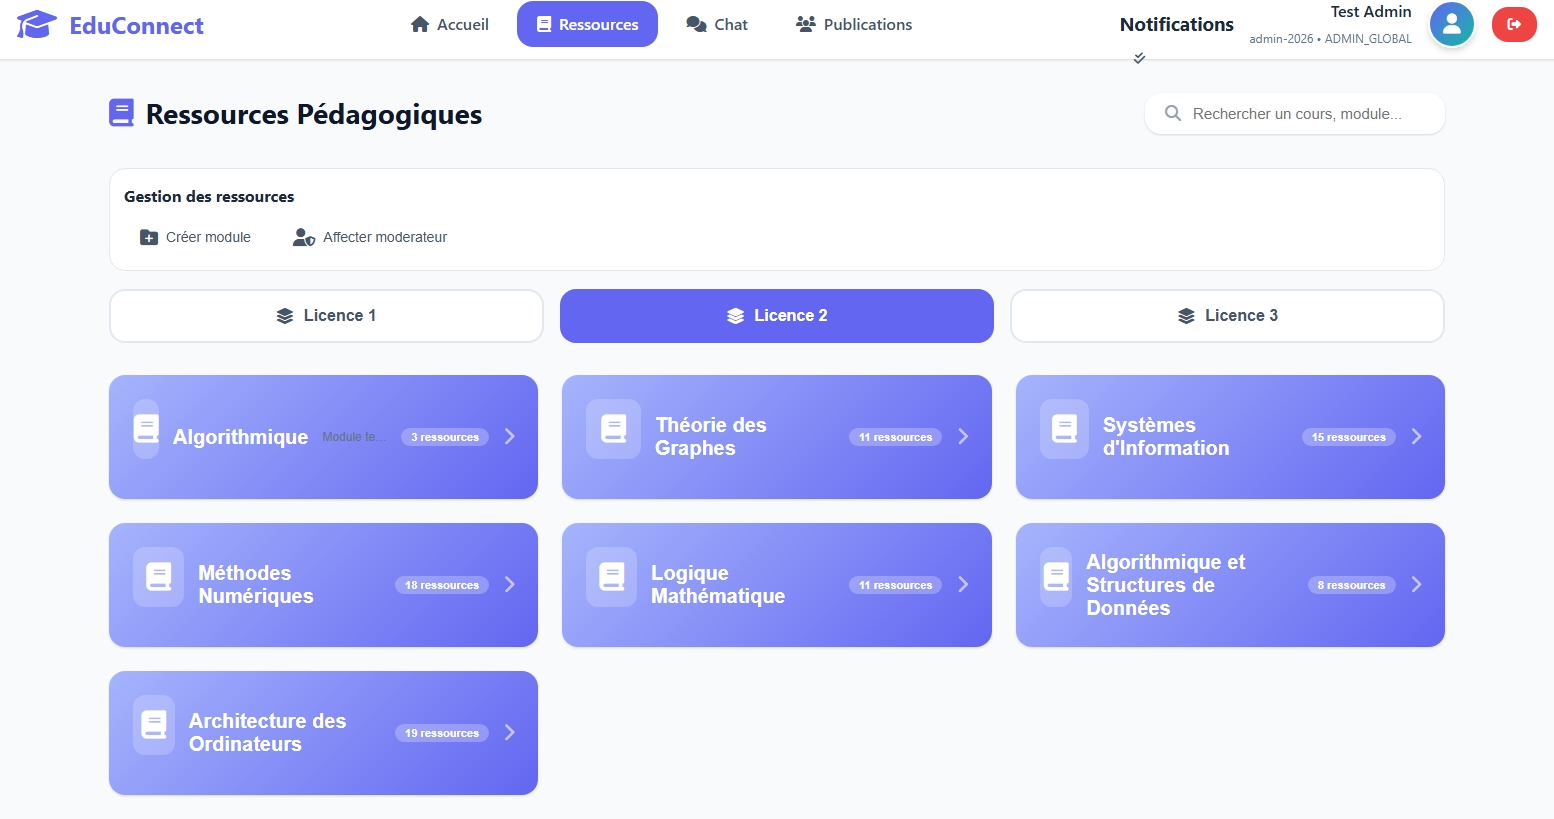
\includegraphics[width=0.85\textwidth]{figures/F1_interface_modules.png}
  \caption{Interface principale d'EduConnect~: navigation par modules (vue liste des modules par niveau).}
  \label{fig:F1}
\end{figure}

%%──────────────────────────
\subsection{Figure~2~---~Capture~: ressources dans un module}

\begin{figurebox}{Figure~2~---~Capture de la page d'un module}
\textbf{Ce que vous devez capturer~:} Une page module avec ses ressources list\'ees par section.

\textbf{Proc\'edure~:}
\begin{enumerate}
  \item Depuis la page des modules, cliquer sur un module existant (ex.~: Algorithmique, R\'eseaux, SGBD).
  \item La page d\'edi\'ee s'affiche avec les sections~: Cours, TD, TP, Examen, Corrig\'e.
  \item Les boutons \textit{Modifier} (bleu) et \textit{Supprimer} (rouge) sont visibles en vue admin~: \textbf{les montrer}.
  \item Capturer en plein \'ecran.
  \item Enregistrer sous~: \texttt{figures/F2\_interface\_ressources.png}
\end{enumerate}
\textbf{Objectif~:} D\'emontrer l'organisation hi\'erarchique Niveau\,$\to$\,Module\,$\to$\,Section\,$\to$\,Ressource avec la gestion CRUD visible.
\end{figurebox}

\begin{figure}[H]
  \centering
  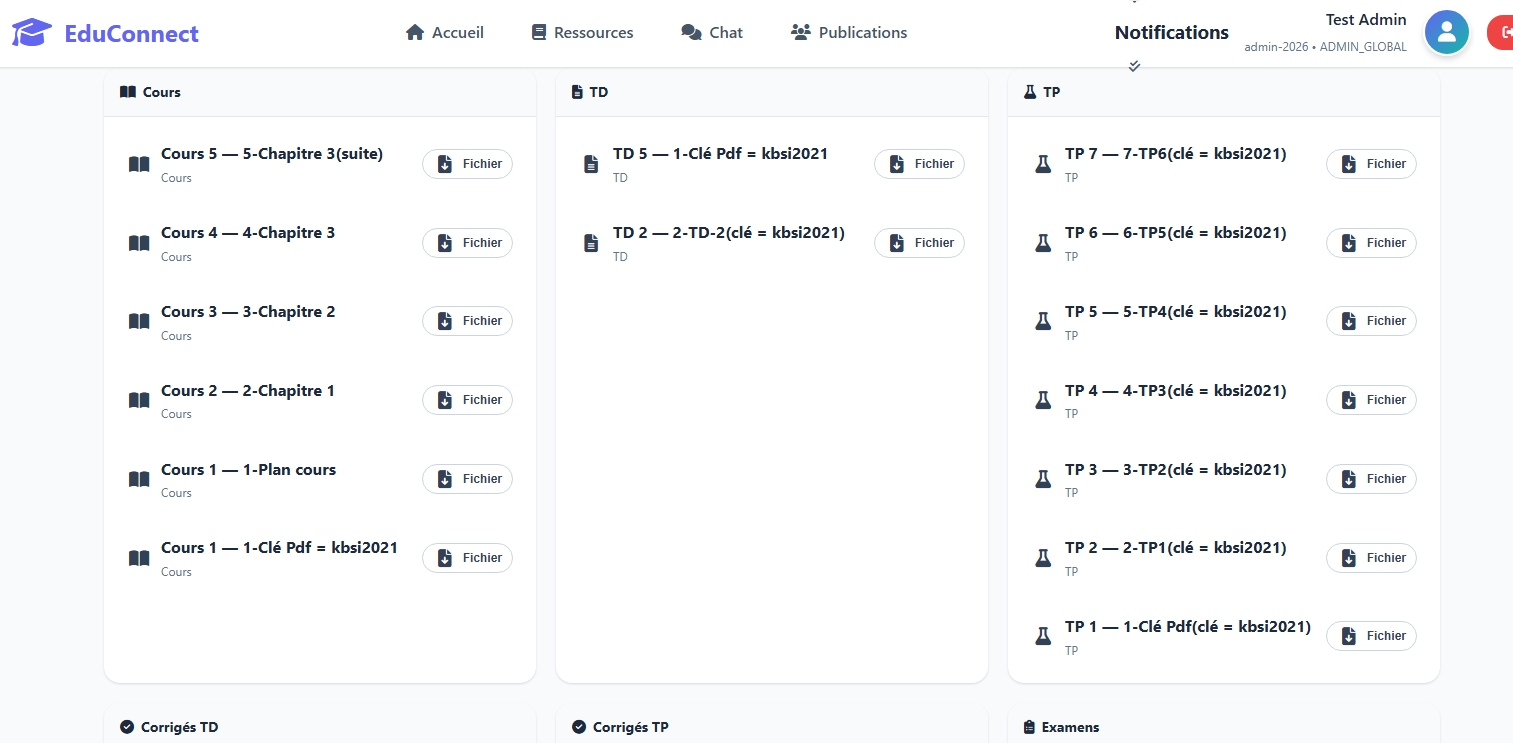
\includegraphics[width=0.85\textwidth]{figures/F2_interface_ressources.png}
  \caption{Interface d'EduConnect~: page d\'edi\'ee d'un module avec ses ressources organis\'ees par section (vue administrateur).}
  \label{fig:F2}
\end{figure}

%%──────────────────────────
\subsection{Figure~3~---~Capture~: publications et chat}

\begin{figurebox}{Figure~3~---~Capture de la couche sociale}
\textbf{Ce que vous devez capturer~:} Le fil de publications et/ou le chat.

\textbf{Proc\'edure~:}
\begin{enumerate}
  \item Cliquer sur \og{}Publications\fg{} dans le menu principal.
  \item Si vide, cr\'eer une publication de test avec quelques commentaires.
  \item Capturer le fil avec au moins une publication visible (titre, contenu, votes, commentaires).
  \item Pour le chat~: ouvrir la messagerie, ouvrir une conversation, capturer.
  \item Enregistrer sous~: \texttt{figures/F3\_interface\_social.png}
\end{enumerate}
\textbf{Objectif~:} D\'emontrer la dimension collaborative d'EduConnect absente de la majorit\'e des LMS classiques.
\end{figurebox}

\begin{figure}[H]
  \centering
  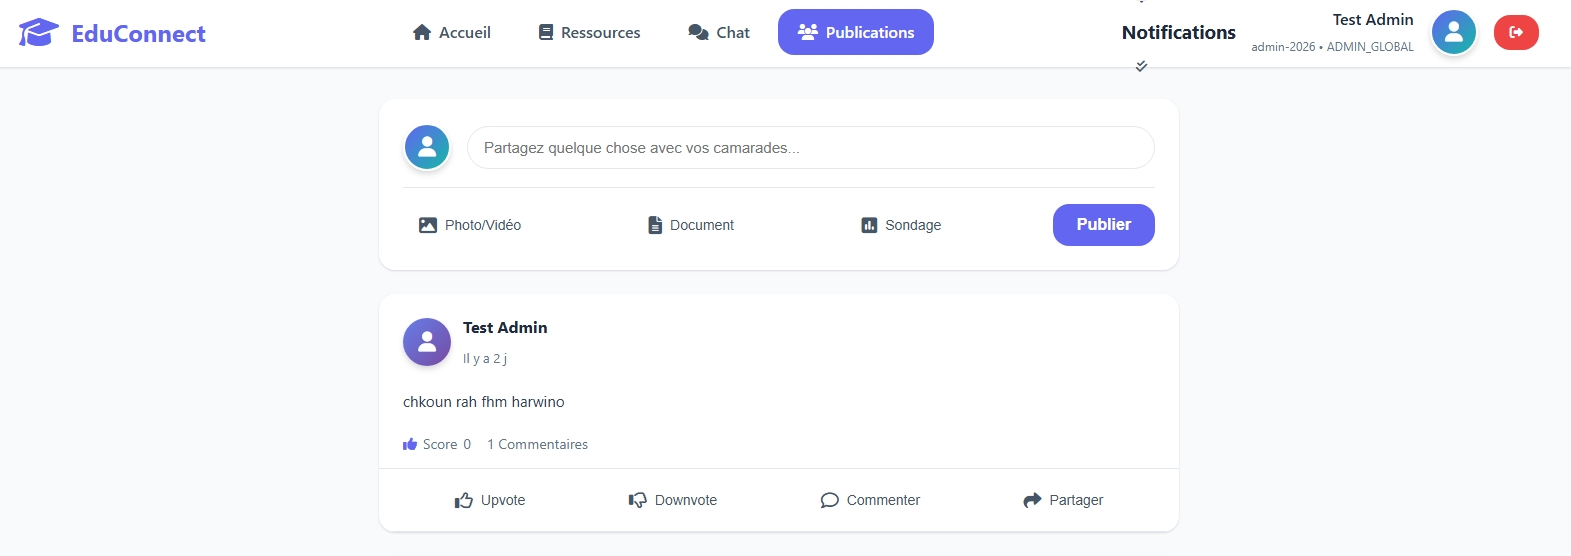
\includegraphics[width=0.85\textwidth]{figures/F3_interface_social.png}
  \caption{Interface d'EduConnect~: fil de publications et chat int\'egr\'es~--- couche sociale de la plateforme.}
  \label{fig:F3}
\end{figure}

%%──────────────────────────────────────────────────────────────────────────────
\section{Conclusion du chapitre}
\label{sec:conclusion}
%%──────────────────────────────────────────────────────────────────────────────

Ce premier chapitre a \'etabli le cadre analytique et conceptuel du projet EduConnect en articulant trois niveaux de lecture compl\'ementaires~: le contexte mondial de la transformation num\'erique de l'enseignement, les besoins sp\'ecifiques du contexte acad\'emique local de l'USTO-MB, et le positionnement d'EduConnect par rapport aux solutions existantes.

L'analyse comparative men\'ee dans la section~\ref{sec:etat_art} d\'emontre qu'aucune des plateformes \'etudi\'ees~--- Moodle, Google Classroom, Microsoft Teams Education, Canvas~--- ne couvre de mani\`ere optimale l'ensemble des exigences identifi\'ees~: navigation module-first, gouvernance \`a trois r\^oles, communication int\'egr\'ee et planification hebdomadaire d\'edi\'ee. Cette convergence de lacunes justifie pleinement la conception d'EduConnect comme solution \textit{ad hoc}, d\'evelopp\'ee sp\'ecifiquement pour le contexte universitaire local.

La suite du m\'emoire approfondit successivement la conception UML (Chapitre~2), l'impl\'ementation technique (Chapitre~3) et l'\'evaluation des r\'esultats (Chapitre~4), en s'appuyant sur le cadre th\'eorique et m\'ethodologique pos\'e dans le pr\'esent chapitre.

%% ═══════════════════════════════════════════════════════════════════════════════
%% CHAPITRE 2 — Analyse, modelisation UML et conception
%% ═══════════════════════════════════════════════════════════════════════════════

\chapter{Analyse des besoins, modelisation UML et conception}

%%──────────────────────────────────────────────────────────────────────────────
\section{Introduction du chapitre}
%%──────────────────────────────────────────────────────────────────────────────

Ce chapitre formalise la traduction de la problematique metier en specifications exploitables pour la realisation logicielle. Il presente successivement l'analyse des besoins, la modelisation UML des interactions, la conception des donnees et les choix architecturaux retenus pour EduConnect.

L'objectif est double: garantir la coherence fonctionnelle de la solution et reduire les risques de derivation durant l'implementation.

%%──────────────────────────────────────────────────────────────────────────────
\section{Analyse des besoins}
%%──────────────────────────────────────────────────────────────────────────────

\subsection{Identification des acteurs}

Quatre acteurs principaux structurent le systeme:
\begin{itemize}
  \item \textbf{Super administrateur}: gouvernance plateforme, ecoles, administrateurs;
  \item \textbf{Administrateur d'ecole}: gestion des utilisateurs, modules, assignations, inscriptions;
  \item \textbf{Formateur}: publication des ressources, suivi des etudiants, sessions live;
  \item \textbf{Etudiant}: consultation des ressources, progression, interactions et lives.
\end{itemize}

\subsection{Besoins fonctionnels majeurs}

\begin{itemize}
  \item authentification securisee et controle d'acces par role;
  \item gestion des modules et de leurs composants pedagogiques (Cours/TD/TP);
  \item workflow de gestion des utilisateurs, assignations et inscriptions;
  \item publication/consultation des ressources pedagogiques;
  \item communication (chat, publications) et suivi de progression;
  \item diffusion de sessions live avec acces cible aux etudiants concernes.
\end{itemize}

\subsection{Besoins non fonctionnels}

\begin{itemize}
  \item securite: JWT, validation des droits, isolation multi-ecole;
  \item performance: API REST reactive, requetes SQL optimisees;
  \item maintenabilite: architecture modulaire frontend/backend;
  \item evolutivite: ajout de nouvelles fonctionnalites sans rupture;
  \item ergonomie: reduction de la surcharge cognitive par role.
\end{itemize}

\subsection{Besoins detailles par acteur}

Afin de garantir une couverture fonctionnelle complete, les besoins ont ete declins acteur par acteur. Cette decomposition facilite la priorisation, la validation des droits et la preparation des tests de recette.

\renewcommand{\arraystretch}{1.35}
\begin{longtable}{|p{2.8cm}|p{4.6cm}|p{4.6cm}|}
\caption{Besoins detailles par acteur}\label{tab:besoins_acteurs}\\
\hline
\rowcolor{ustoblue}
\textcolor{white}{\textbf{Acteur}} &
\textcolor{white}{\textbf{Besoins prioritaires}} &
\textcolor{white}{\textbf{Valeur attendue}} \\
\hline
Super administrateur &
Creer les ecoles, nommer les administrateurs, superviser la plateforme globale. &
Gouvernance transverse et maitrise des droits inter-etablissements. \\
\hline
Administrateur d'ecole &
Gerer comptes, modules, assignations, inscriptions, calendrier pedagogique. &
Pilotage quotidien de l'activite academique et reduction des taches manuelles. \\
\hline
Formateur &
Publier ressources, organiser Cours/TD/TP, lancer des sessions live, suivre les etudiants. &
Production pedagogique structuree et interaction rapide avec les apprenants. \\
\hline
Etudiant &
Consulter ressources, suivre les annonces, acceder aux lives, interagir via chat/publications. &
Acces clair aux contenus et meilleure continuite d'apprentissage. \\
\hline
\end{longtable}

%%──────────────────────────────────────────────────────────────────────────────
\section{Modelisation UML}
%%──────────────────────────────────────────────────────────────────────────────

\subsection{Diagramme de cas d'utilisation}

Les cas d'utilisation centraux incluent:
\begin{itemize}
  \item \textbf{Administrer la plateforme}: creer ecoles et administrateurs;
  \item \textbf{Administrer une ecole}: gerer utilisateurs, modules, assignations et inscriptions;
  \item \textbf{Produire et diffuser}: uploader et organiser les ressources;
  \item \textbf{Apprendre et interagir}: consulter, telecharger, completer des ressources;
  \item \textbf{Animer en direct}: creer, demarrer et terminer une session live.
\end{itemize}

\begin{figurebox}{Cas d'utilisation global EduConnect}
Inserez ici le diagramme de cas d'utilisation general du systeme (acteurs + cas + relations include/extend).
\end{figurebox}

\subsection{Diagrammes de sequence a mettre a jour}

Conformement a votre demande de mise a jour des diagrammes, les scenarios prioritaires sont:
\begin{itemize}
  \item \textbf{Sequence 1}: creation d'un module et affectation d'un formateur;
  \item \textbf{Sequence 2}: inscription d'un etudiant a un module;
  \item \textbf{Sequence 3}: publication d'une ressource pedagogique;
  \item \textbf{Sequence 4}: cycle d'une session live (creation, passage LIVE, affichage etudiant, cloture).
\end{itemize}

\begin{figurebox}{Sequence 4 — Session live}
Participants recommandes: Formateur, Interface React, API Express, LiveSession Model, PostgreSQL, Dashboard Etudiant.
\end{figurebox}

\subsection{Diagramme de classes conceptuel}

Le modele conceptuel s'articule autour de classes principales:
\begin{itemize}
  \item \texttt{User} (roles, school, profil),
  \item \texttt{Module} (code, nom, niveau, composants),
  \item \texttt{Assignment} (formateur-module-type),
  \item \texttt{Enrollment} (etudiant-module-statut),
  \item \texttt{Resource} (categorie, fichier, statut),
  \item \texttt{LiveSession} (lien, statut, horodatages).
\end{itemize}

\begin{figurebox}{Diagramme de classes EduConnect}
Montrer cardinalites, cles primaires/etrangeres et contraintes metier (roles, statuts, scopes).
\end{figurebox}

%%──────────────────────────────────────────────────────────────────────────────
\section{Scenarios metier detailles}
%%──────────────────────────────────────────────────────────────────────────────

Cette section formalise les principaux parcours metier sous forme textuelle. Elle complete les diagrammes UML et sert de reference pour la validation fonctionnelle.

\subsection{Scenario A: creation d'un module et affectation d'un formateur}

\textbf{Preconditions:} l'administrateur est authentifie et dispose des droits de gestion de son ecole.

\textbf{Flux principal:}
\begin{enumerate}
  \item l'administrateur cree un module (code, intitule, niveau, semestre);
  \item le systeme verifie l'unicite du code dans le contexte de l'ecole;
  \item l'administrateur affecte un formateur principal et, si necessaire, des formateurs secondaires;
  \item le systeme notifie les formateurs concernes et rend le module visible selon les droits.
\end{enumerate}

\textbf{Postconditions:} le module est actif et pret a recevoir des ressources pedagogiques.

\subsection{Scenario B: inscription d'un etudiant}

\textbf{Preconditions:} etudiant cree dans le systeme et module disponible.

\textbf{Flux principal:}
\begin{enumerate}
  \item l'administrateur selectionne l'etudiant et le module cible;
  \item l'API valide l'appartenance a la meme ecole et l'absence de doublon;
  \item l'inscription est enregistree avec statut initial;
  \item l'etudiant voit immediatement le module dans son espace personnel.
\end{enumerate}

\textbf{Postconditions:} l'etudiant accede aux ressources et annonces du module inscrit.

\subsection{Scenario C: session live de bout en bout}

\textbf{Preconditions:} le formateur est assigne au module et dispose d'un lien de reunion valide.

\textbf{Flux principal:}
\begin{enumerate}
  \item creation d'une session avec statut \texttt{SCHEDULED};
  \item passage en statut \texttt{LIVE} au demarrage;
  \item affichage en temps reel cote etudiant sur dashboard et page module;
  \item cloture avec passage \texttt{ENDED} et horodatage de fin.
\end{enumerate}

\textbf{Postconditions:} la session reste tracable pour reporting et audit pedagogique.

%%──────────────────────────────────────────────────────────────────────────────
\section{Conception des donnees}
%%──────────────────────────────────────────────────────────────────────────────

\subsection{Principes de conception}

Le schema relationnel repose sur:
\begin{itemize}
  \item normalisation des entites pour reduire la redondance;
  \item contraintes d'integrite (PK/FK, \texttt{CHECK}, \texttt{NOT NULL});
  \item journalisation temporelle (\texttt{created\_at}, \texttt{started\_at}, \texttt{ended\_at});
  \item indexation des colonnes critiques (recherche et tri par statut/date).
\end{itemize}

\subsection{Extension live\_sessions}

L'ajout de la table \texttt{live\_sessions} formalise la fonctionnalite de live pedagogique.
Les attributs cle incluent:
\begin{itemize}
  \item \texttt{formateur\_id}, \texttt{module\_id}, \texttt{meeting\_link};
  \item \texttt{status} dans \{SCHEDULED, LIVE, ENDED\};
  \item \texttt{scheduled\_at}, \texttt{started\_at}, \texttt{ended\_at}.
\end{itemize}

Ce schema garantit la traçabilite des sessions et facilite le filtrage par role.

\subsection{Regles de gestion et contraintes de donnees}

Pour renforcer la fiabilite metier, les regles suivantes ont ete retenues:
\begin{itemize}
  \item un module appartient a une seule ecole et son code y est unique;
  \item un etudiant ne peut pas etre inscrit deux fois au meme module;
  \item seuls les formateurs assignes peuvent creer ou modifier des ressources du module;
  \item une session live ne peut passer a \texttt{LIVE} que depuis l'etat \texttt{SCHEDULED};
  \item l'etat \texttt{ENDED} est terminal et interdit toute reprise de session;
  \item toute action d'administration doit etre rattachee a un utilisateur authentifie.
\end{itemize}

%%──────────────────────────────────────────────────────────────────────────────
\section{Architecture logicielle retenue}
%%──────────────────────────────────────────────────────────────────────────────

\subsection{Vue d'ensemble}

L'architecture suit un modele client-serveur decouple:
\begin{itemize}
  \item \textbf{Frontend}: React (SPA), routage protege, composants par role;
  \item \textbf{Backend}: Node.js/Express, controleurs REST, services metier, middlewares;
  \item \textbf{Base de donnees}: PostgreSQL, migrations SQL versionnees.
\end{itemize}

\subsection{Justification des choix}

\begin{itemize}
  \item React facilite une UX dynamique et modulaire;
  \item Express accelere la construction d'API REST maintenables;
  \item PostgreSQL assure robustesse transactionnelle et performance relationnelle;
  \item JWT permet une authentification stateless adaptee a une architecture API.
\end{itemize}

\begin{figurebox}{Architecture technique globale}
Inserez un schema en couches: UI React -> API Express -> Services/Models -> PostgreSQL.
\end{figurebox}

%%──────────────────────────────────────────────────────────────────────────────
\section{Risque projet et criteres d'acceptation}
%%──────────────────────────────────────────────────────────────────────────────

\subsection{Risques principaux}

\begin{itemize}
  \item complexite des droits multi-roles;
  \item derive UX en cas de surcharge d'ecrans admin;
  \item dette technique si l'evolution n'est pas guidee par conventions.
\end{itemize}

\subsection{Criteres d'acceptation}

\begin{itemize}
  \item chaque role accede uniquement aux fonctionnalites autorisees;
  \item les workflows critiques (module, inscription, live) sont executables de bout en bout;
  \item l'interface reste lisible sur desktop et mobile;
  \item les donnees critiques sont tracables et coherentes en base.
\end{itemize}

%%──────────────────────────────────────────────────────────────────────────────
\section{Matrice de tracabilite besoins-cas-tests}
%%──────────────────────────────────────────────────────────────────────────────

La tracabilite relie explicitement chaque besoin a un cas d'utilisation et a un test de validation. Cette pratique reduit le risque d'oublis fonctionnels durant la recette.

\renewcommand{\arraystretch}{1.35}
\begin{longtable}{|p{2.2cm}|p{4.1cm}|p{3.5cm}|p{3.6cm}|}
\caption{Matrice de tracabilite fonctionnelle}\label{tab:traceabilite}\\
\hline
\rowcolor{ustoblue}
\textcolor{white}{\textbf{Exigence}} &
\textcolor{white}{\textbf{Description}} &
\textcolor{white}{\textbf{Cas UML associe}} &
\textcolor{white}{\textbf{Validation attendue}} \\
\hline
OS1 & Centraliser ressources pedagogiques & Produire et diffuser & Ressources accessibles par module/composant \\
\hline
OS2 & Authentification et autorisation par roles & Administrer la plateforme/ecole & Acces refuses hors privileges \\
\hline
OS3 & Communication integree & Apprendre et interagir & Publications/chat operationnels \\
\hline
OS4 & Notifications des evenements & Apprendre et interagir & Notification visible apres evenement \\
\hline
OS5 & Planification hebdomadaire & Administrer une ecole & Activites affichees par semaine \\
\hline
OS6 & Tracabilite des operations & Administrer la plateforme/ecole & Historique coherent en base \\
\hline
Live & Session synchrone encadree & Animer en direct & Etats SCHEDULED/LIVE/ENDED conformes \\
\hline
\end{longtable}

%%──────────────────────────────────────────────────────────────────────────────
\section{Conclusion du chapitre}
%%──────────────────────────────────────────────────────────────────────────────

Ce chapitre a etabli le pont entre besoins metier et solution technique. L'analyse fonctionnelle, les modeles UML et la conception de donnees offrent un cadre methodologique solide pour la realisation. Le chapitre suivant detaille l'implementation concrete, les choix de deploiement et les resultats de validation obtenus sur la plateforme.

%% ═══════════════════════════════════════════════════════════════════════════════
%% CHAPITRE 3 — Realisation, deploiement et validation
%% ═══════════════════════════════════════════════════════════════════════════════

\chapter{Realisation technique, deploiement et validation}

%%──────────────────────────────────────────────────────────────────────────────
\section{Introduction du chapitre}
%%──────────────────────────────────────────────────────────────────────────────

Apres la phase d'analyse et de conception, ce chapitre presente la realisation effective d'EduConnect. Il decrit l'environnement de developpement, l'implementation des modules fonctionnels, l'integration de la fonctionnalite live, puis les tests de validation.

%%──────────────────────────────────────────────────────────────────────────────
\section{Environnement technologique}
%%──────────────────────────────────────────────────────────────────────────────

\subsection{Stack technique}

\begin{itemize}
  \item Frontend: React (SPA), React Router, Axios;
  \item Backend: Node.js, Express, middlewares de securite;
  \item Base de donnees: PostgreSQL;
  \item Authentification: JWT;
  \item Outils: VS Code, Git, scripts de migration SQL.
\end{itemize}

\subsection{Organisation du code}

Le projet est structure en deux blocs:
\begin{itemize}
  \item \textbf{frontend}: pages par role, composants UI, services API;
  \item \textbf{backend}: routes, controleurs, modeles, services metier.
\end{itemize}

Cette separation facilite la maintenabilite et l'evolution incrémentale.

\subsection{Configuration d'execution}

Le fonctionnement d'EduConnect repose sur une separation claire des environnements de developpement et de production.
\begin{itemize}
  \item \textbf{Variables d'environnement}: configuration des ports, URL API, secrets JWT et acces base de donnees;
  \item \textbf{Parametres de securite}: expiration des jetons, politique CORS et validation des entrees;
  \item \textbf{Scripts de lancement}: demarrage independant frontend/backend pour faciliter le debug par couche.
\end{itemize}

Cette configuration limite les regressions entre postes de developpement et prepare la transition vers un deploiement reproductible.

%%──────────────────────────────────────────────────────────────────────────────
\section{Architecture d'execution et flux applicatifs}
%%──────────────────────────────────────────────────────────────────────────────

\subsection{Flux client-serveur principal}

Le cycle d'une requete suit les etapes suivantes:
\begin{enumerate}
  \item emission d'une action utilisateur depuis l'interface React;
  \item appel HTTP via service API avec jeton JWT si route protegee;
  \item passage par les middlewares de controle (authentification/autorisation/validation);
  \item execution de la logique metier dans les controleurs et services;
  \item acces PostgreSQL et retour JSON structure vers le frontend.
\end{enumerate}

\subsection{Gestion des erreurs}

Une strategie de gestion d'erreurs a ete appliquee pour garantir un comportement previsible:
\begin{itemize}
  \item codes HTTP coherents (401, 403, 404, 422, 500);
  \item messages explicites cote interface pour guider l'utilisateur;
  \item journalisation des erreurs serveur afin de faciliter le diagnostic.
\end{itemize}

%%──────────────────────────────────────────────────────────────────────────────
\section{Implementation des fonctionnalites principales}
%%──────────────────────────────────────────────────────────────────────────────

\subsection{Gestion des utilisateurs et des roles}

Le systeme applique un controle d'acces strict par role global et contexte ecole. Les routes critiques sont protegees par authentification et verification de privileges.

\subsection{Gestion pedagogique par module}

La plateforme gere:
\begin{itemize}
  \item creation/modification des modules;
  \item structuration par composants (Cours/TD/TP);
  \item assignation des formateurs (principal/simple);
  \item inscriptions etudiants et suivi des ressources.
\end{itemize}

\subsection{Communication et collaboration}

Les utilisateurs disposent d'espaces de communication (chat/publications) afin de fluidifier les interactions pedagogiques et l'entraide.

\subsection{Traçabilite des operations metier}

Les operations critiques (creation module, assignation, inscription, changements d'etat live) sont realisees via des points d'entree explicites cote API. Cette structuration permet:
\begin{itemize}
  \item de verifier les droits avant toute modification en base;
  \item de conserver une chronologie claire des changements;
  \item de faciliter les audits fonctionnels en phase de validation.
\end{itemize}

%%──────────────────────────────────────────────────────────────────────────────
\section{Implementation de la fonctionnalite Live}
%%──────────────────────────────────────────────────────────────────────────────

\subsection{Conception metier du live}

La fonctionnalite live repose sur un cycle de vie simple:
\begin{itemize}
  \item \texttt{SCHEDULED}: session planifiee;
  \item \texttt{LIVE}: session en direct;
  \item \texttt{ENDED}: session terminee.
\end{itemize}

Le formateur cree une session avec un lien de reunion (Zoom/Meet/Teams), puis controle son etat. Les etudiants concernes voient automatiquement les sessions actives ou programmees.

\subsection{Realisation backend}

Les points d'API implementes couvrent:
\begin{itemize}
  \item creation et consultation des sessions du formateur;
  \item transition d'etat (demarrer/terminer);
  \item suppression d'une session;
  \item recuperation des lives pertinents cote etudiant.
\end{itemize}

Pour renforcer la robustesse, le backend verifie egalement la coherence des transitions d'etat. Une session ne peut pas passer directement de \texttt{SCHEDULED} a \texttt{ENDED} sans passage par \texttt{LIVE}, sauf action d'annulation explicite.

\subsection{Realisation frontend}

Deux integrations ont ete realisees:
\begin{itemize}
  \item page dediee formateur pour gerer les sessions live;
  \item widget dashboard etudiant affichant les lives actifs/programmes.
\end{itemize}

Cette implementation assure une liaison directe entre la planification enseignant et l'experience apprenant.

%%──────────────────────────────────────────────────────────────────────────────
\section{Securite applicative et protection des donnees}
%%──────────────────────────────────────────────────────────────────────────────

La securite a ete traitee comme une contrainte transversale, non comme une fonctionnalite secondaire.

\subsection{Authentification et autorisation}

\begin{itemize}
  \item authentification par jeton JWT signe;
  \item verification des droits selon role global et contexte ecole;
  \item protection des routes d'administration et d'ecriture.
\end{itemize}

\subsection{Validation des donnees et reduction des risques}

\begin{itemize}
  \item validation serveur des champs obligatoires et formats attendus;
  \item controles metier sur les relations formateur-module-etudiant;
  \item limitation des effets de bord grace a des flux CRUD explicites.
\end{itemize}

\subsection{Protection operationnelle minimale}

Les mesures suivantes ont ete appliquees dans le cadre du projet:
\begin{itemize}
  \item restriction des operations sensibles aux profils autorises;
  \item gestion de l'expiration des sessions d'authentification;
  \item usage de configurations separees pour eviter l'exposition de secrets en code source.
\end{itemize}

%%──────────────────────────────────────────────────────────────────────────────
\section{Deploiement et exploitation}
%%──────────────────────────────────────────────────────────────────────────────

\subsection{Strategie de deploiement retenue}

Le deploiement est organise en trois niveaux:
\begin{itemize}
  \item \textbf{Developpement local}: iteration rapide des fonctionnalites;
  \item \textbf{Pre-production}: verification des parcours critiques avec donnees de test;
  \item \textbf{Production pilote}: ouverture controlee aux utilisateurs reels.
\end{itemize}

\subsection{Sauvegarde et continuite}

Afin de limiter le risque de perte de donnees:
\begin{itemize}
  \item des sauvegardes periodiques de la base PostgreSQL sont planifiees;
  \item les scripts de restauration sont documentes pour une reprise rapide;
  \item les evolutions schema sont tracees via scripts SQL versionnes.
\end{itemize}

\subsection{Supervision et maintenance}

La maintenance applicative suit une boucle continue:
\begin{enumerate}
  \item collecte des incidents et retours utilisateurs;
  \item priorisation selon impact pedagogique et frequence;
  \item correction, verification et redeploiement cible.
\end{enumerate}

%%──────────────────────────────────────────────────────────────────────────────
\section{Ameliorations UX realisees}
%%──────────────────────────────────────────────────────────────────────────────

Une passe UX a ete effectuee pour reduire la surcharge cognitive:
\begin{itemize}
  \item affichage des modules admin en grille lisible;
  \item filtres metier (niveau, role, module, type) sur ecrans admin;
  \item suppression de colonnes peu utiles (exemple: ID) dans les tableaux;
  \item enrichissement visuel des tableaux de bord et cartes de suivi;
  \item integration visuelle du bloc live sur les dashboards concernes.
\end{itemize}

%%──────────────────────────────────────────────────────────────────────────────
\section{Validation fonctionnelle}
%%──────────────────────────────────────────────────────────────────────────────

\subsection{Jeux d'essais}

Les validations ont ete conduites sur des comptes de test multi-roles:
\begin{itemize}
  \item administration (super-admin et admin ecole),
  \item formateurs,
  \item etudiants.
\end{itemize}

\subsection{Resultats observes}

\begin{itemize}
  \item authentification et redirections par role conformes;
  \item workflows de gestion (module/assignation/inscription) operationnels;
  \item fonctionnalite live testee de bout en bout (creation -> LIVE -> affichage etudiant);
  \item compilation frontend validee sans erreurs bloquantes sur les ecrans modifies.
\end{itemize}

\subsection{Tableau synthetique de validation}

\renewcommand{\arraystretch}{1.3}
\begin{table}[H]
\centering
\caption{Synthese des tests fonctionnels principaux}
\label{tab:tests_ch3}
\begin{tabular}{|p{4.3cm}|p{3.2cm}|p{2.4cm}|p{2.6cm}|}
\hline
\rowcolor{ustoblue}
\textcolor{white}{Scenario teste} &
\textcolor{white}{Role principal} &
\textcolor{white}{Statut} &
\textcolor{white}{Observation} \\
\hline
Creation/edition module & Admin ecole & Valide & Workflow stable \\
\hline
Assignation formateur & Admin ecole & Valide & Regles de droits respectees \\
\hline
Inscription etudiant & Admin ecole & Valide & Visibilite module immediate \\
\hline
Publication ressource & Formateur & Valide & Organisation Cours/TD/TP conforme \\
\hline
Session live complete & Formateur + Etudiant & Valide & Etats SCHEDULED/LIVE/ENDED coherents \\
\hline
Consultation ressources & Etudiant & Valide & Parcours fluide et lisible \\
\hline
\end{tabular}
\end{table}

\subsection{Limites actuelles}

\begin{itemize}
  \item les liens live sont externes (pas de visio embarquee native);
  \item la metrologie produit (analytics avances) reste a industrialiser;
  \item certains tests automatises restent a renforcer pour le passage a l'echelle.
\end{itemize}

\subsection{Axes d'amelioration technique court terme}

\begin{itemize}
  \item augmenter la couverture de tests automatises sur les routes critiques;
  \item introduire des indicateurs de performance (latence API, erreurs par endpoint);
  \item renforcer la documentation d'exploitation pour faciliter l'onboarding technique.
\end{itemize}

%%──────────────────────────────────────────────────────────────────────────────
\section{Synthese et perspectives techniques}
%%──────────────────────────────────────────────────────────────────────────────

La realisation confirme la faisabilite technique du socle EduConnect et sa capacite a supporter des usages reels multi-acteurs. Les evolutions prioritaires envisagees sont:
\begin{itemize}
  \item observabilite avancee (logs metier, tableaux de supervision),
  \item automatisation QA (tests integration/e2e),
  \item optimisation des performances sur charge elevee.
\end{itemize}

%%──────────────────────────────────────────────────────────────────────────────
\section{Conclusion du chapitre}
%%──────────────────────────────────────────────────────────────────────────────

Ce chapitre a decrit l'implementation concrete d'EduConnect et les validations associees. Les resultats montrent une plateforme fonctionnelle, evolutive et coherente avec les objectifs du projet. Le chapitre suivant complete cette analyse par la dimension entrepreneuriale: modele economique, SWOT et strategie de croissance startup.

%% ═══════════════════════════════════════════════════════════════════════════════
%% CHAPITRE 4 — Modele economique, positionnement startup et analyse SWOT
%% ═══════════════════════════════════════════════════════════════════════════════

\chapter{Modele economique, positionnement startup et analyse SWOT}

%%──────────────────────────────────────────────────────────────────────────────
\section{Introduction du chapitre}
%%──────────────────────────────────────────────────────────────────────────────

Dans les chapitres precedents, nous avons expose le contexte, la problematique, puis les choix techniques et fonctionnels qui structurent la plateforme EduConnect. Le present chapitre deplace l'analyse vers la viabilite entrepreneuriale du projet. L'objectif est de verifier que la proposition de valeur n'est pas uniquement techniquement realisable, mais egalement economiquement soutenable dans un contexte de startup EdTech.

Ce chapitre poursuit quatre finalites. Premierement, formaliser un modele economique coherent a travers le \textit{Business Model Canvas} (BMC)\cite{osterwalder2010bmc}. Deuxiemement, evaluer la position strategique de la startup au moyen d'une matrice SWOT\cite{kotler2017marketing}. Troisiemement, proposer des scenarios de monetisation et des indicateurs de pilotage. Quatriemement, definir une feuille de route de croissance progressive adaptee au contexte universitaire local.

%%──────────────────────────────────────────────────────────────────────────────
\section{Vision startup et hypotheses de depart}
%%──────────────────────────────────────────────────────────────────────────────

EduConnect est envisage comme une startup B2B2C EdTech. Le coeur du modele consiste a contractualiser avec les etablissements (B2B), tout en delivrant de la valeur directe aux formateurs et etudiants (B2C indirect). Ce positionnement permet de traiter simultanement les enjeux institutionnels (gouvernance, securite, traçabilite) et les usages quotidiens (cours, TD, TP, lives, communication, suivi).

\subsection{Probleme marche adresse}

Les structures universitaires et ecoles privees font face a trois contraintes recurrentes:
\begin{itemize}
  \item dispersion des ressources pedagogiques entre plusieurs canaux non gouvernes;
  \item manque de pilotage centralise (droits, validations, historique, reporting);
  \item faible qualite de l'experience numerique pour les enseignants et apprenants.
\end{itemize}

\subsection{Hypotheses business initiales}

\begin{itemize}
  \item Le besoin de centralisation pedagogique est suffisamment critique pour justifier un abonnement institutionnel.
  \item Les etablissements privilegient une solution locale, configurable et conforme aux exigences de gouvernance.
  \item Les fonctionnalites differenciantes (multi-ecole, workflow de validation, sessions live, suivi) augmentent le taux d'adoption interne.
  \item Un deploiement progressif par pilote (une ecole, puis extension) reduit le risque commercial et technique.
\end{itemize}

\subsection{Hypotheses de validation produit-marche}

Au-dela des hypotheses business, trois hypotheses de validation produit-marche sont retenues:
\begin{itemize}
  \item \textbf{H1 --- Adoption formateur}: au moins 70\,\% des formateurs pilotes publient au minimum une ressource par semaine.
  \item \textbf{H2 --- Activation etudiant}: au moins 60\,\% des etudiants connectes consultent activement les ressources sur une periode de 30 jours.
  \item \textbf{H3 --- Valeur institutionnelle}: l'administration confirme une reduction perceptible du temps de coordination pedagogique.
\end{itemize}

Ces hypotheses servent de base a la priorisation roadmap et a la decision de passage a l'echelle.

%%──────────────────────────────────────────────────────────────────────────────
\section{Analyse du marche et positionnement concurrentiel}
%%──────────────────────────────────────────────────────────────────────────────

Le positionnement d'EduConnect ne se limite pas a une comparaison fonctionnelle avec les LMS etablis. Il repose sur une strategie de specialisation locale, orientee gouvernance pedagogique et simplicite d'usage.

\subsection{Lecture TAM / SAM / SOM}

\begin{itemize}
  \item \textbf{TAM (Total Addressable Market)}: l'ensemble des etablissements d'enseignement superieur et structures de formation pouvant numeriser leurs processus pedagogiques.
  \item \textbf{SAM (Serviceable Available Market)}: les institutions disposant d'une maturite numerique minimale et d'un besoin explicite de plateforme unifiee.
  \item \textbf{SOM (Serviceable Obtainable Market)}: la part realiste atteignable a court terme via pilotes regionaux et effet de recommandation inter-etablissements.
\end{itemize}

Cette lecture permet d'eviter une surprojection commerciale et d'ancrer les objectifs de croissance dans une trajectoire executable.

\subsection{Differenciation concurrentielle}

Les concurrents generalistes couvrent un spectre large, mais avec une adaptation locale limitee. EduConnect se differencie sur:
\begin{itemize}
  \item la gouvernance fine multi-ecole et multi-roles;
  \item la structuration pedagogique native Cours/TD/TP;
  \item la proximite terrain pour l'accompagnement et l'iteration produit;
  \item la capacite d'implementation progressive sans rupture organisationnelle.
\end{itemize}

\renewcommand{\arraystretch}{1.3}
\begin{table}[H]
\centering
\caption{Positionnement concurrentiel simplifie}
\label{tab:positionnement_concurrentiel}
\begin{tabular}{|p{3.0cm}|p{3.2cm}|p{3.2cm}|p{3.2cm}|}
\hline
\rowcolor{ustoblue}
\textcolor{white}{Solution} & \textcolor{white}{Adaptation locale} & \textcolor{white}{Gouvernance pedagogique} & \textcolor{white}{Accompagnement} \\
\hline
LMS internationaux & Moyenne a faible & Bonne mais generaliste & Standardise \\
\hline
Outils bureautiques + chat & Faible & Fragmentee & Informel \\
\hline
EduConnect & Elevee & Native au contexte metier & Proximite + iteration \\
\hline
\end{tabular}
\end{table}

%%──────────────────────────────────────────────────────────────────────────────
\section{Business Model Canvas d'EduConnect}
%%──────────────────────────────────────────────────────────────────────────────

Le BMC formalise les neuf blocs strategiques de la startup\cite{osterwalder2010bmc}.

\subsection{Segments de clients}

EduConnect cible quatre segments prioritaires:
\begin{itemize}
  \item ecoles superieures et universites (public/privé) cherchant une plateforme pedagogique gouvernee;
  \item administrations pedagogiques (direction, scolarite, responsables filiere);
  \item corps enseignant (formateurs principaux et simples);
  \item etudiants, utilisateurs finaux de l'experience d'apprentissage.
\end{itemize}

\subsection{Proposition de valeur}

La proposition de valeur s'articule autour de six axes:
\begin{itemize}
  \item centralisation des contenus par niveau, module et composant (Cours/TD/TP);
  \item gouvernance fine des acces par roles et ecoles;
  \item interactions pedagogiques integrees (chat, ressources, lives, notifications);
  \item reduction de la surcharge cognitive via une interface structuree;
  \item visibilite admin avec tableaux de bord et actions rapides;
  \item architecture evolutive orientee startup (MVP, iterations, extension multi-tenant).
\end{itemize}

\subsection{Canaux}

\begin{itemize}
  \item canal direct: demonstrations, POC et pilotes dans les etablissements;
  \item canal relationnel: reseau universitaire, enseignants relais, bouche-a-oreille;
  \item canal digital: site vitrine, documentation, supports video de prise en main;
  \item canal partenarial: incubateurs, associations EdTech, acteurs institutionnels.
\end{itemize}

\subsection{Relations clients}

\begin{itemize}
  \item accompagnement de lancement (onboarding admin et formateurs);
  \item support fonctionnel continu (FAQ, tickets, sessions de formation);
  \item co-construction produit (collecte feedback, roadmap trimestrielle);
  \item contrats annuels avec points de revues periodiques.
\end{itemize}

\subsection{Flux de revenus}

Le modele de revenus privilegie l'abonnement institutionnel annuel:
\begin{itemize}
  \item formule \textbf{Starter}: petite ecole, fonctions essentielles;
  \item formule \textbf{Growth}: multi-filieres, reporting avance, priorite support;
  \item formule \textbf{Enterprise}: forte volumetrie, SLA, personnalisation avancee.
\end{itemize}

Des revenus complementaires peuvent etre ajoutes: formation premium, migration de donnees, developpements specifiques, et support etendu.

\subsection{Ressources cles}

\begin{itemize}
  \item equipe produit (developpement full-stack, QA, design UX);
  \item infrastructure cloud/serveur et base PostgreSQL;
  \item bibliotheque de composants et architecture API;
  \item savoir-faire pedagogique et connaissance du terrain universitaire.
\end{itemize}

\subsection{Activites cles}

\begin{itemize}
  \item developpement et maintenance applicative;
  \item securisation et supervision de la plateforme;
  \item deploiement, parametrage et support client;
  \item analyse d'usage et priorisation roadmap.
\end{itemize}

\subsection{Partenaires cles}

\begin{itemize}
  \item etablissements pilotes (co-validation des usages);
  \item hebergeurs/infrastructure cloud;
  \item ecosysteme startup (incubateurs, mentors, experts juridiques);
  \item partenaires de formation et d'integration.
\end{itemize}

\subsection{Structure de couts}

\begin{itemize}
  \item couts techniques: hebergement, sauvegarde, monitoring, securite;
  \item couts humains: developpement, support, commercial, pilotage produit;
  \item couts operationnels: deplacements, documentation, formation clients;
  \item couts d'acquisition: demos, communication, prospection.
\end{itemize}

\subsection{Synthese du BMC}

\renewcommand{\arraystretch}{1.45}
\begin{longtable}{|>{\bfseries\raggedright\arraybackslash}p{3.2cm}|p{10.2cm}|}
\caption{Synthese du Business Model Canvas d'EduConnect}
\label{tab:bmc_edconnect} \\
\hline
\rowcolor{ustoblue}
\textcolor{white}{Bloc} & \textcolor{white}{Elements principaux} \\
\hline
Segments clients & Universites/ecoles, administration pedagogique, formateurs, etudiants \\
\hline
Proposition de valeur & Plateforme pedagogique unifiee, gouvernance par roles, modules Cours/TD/TP, live et collaboration \\
\hline
Canaux & Pilotes institutionnels, reseau universitaire, canal digital, partenariats \\
\hline
Relations clients & Onboarding, support continu, co-construction produit, revues periodiques \\
\hline
Revenus & Abonnements annuels (Starter, Growth, Enterprise), services premium \\
\hline
Ressources cles & Equipe tech/produit, infrastructure, architecture logicielle, expertise metier \\
\hline
Activites cles & Dev/maintenance, securite, support, deploiement, analyse d'usage \\
\hline
Partenaires cles & Ecoles pilotes, hebergeurs, ecosysteme startup, partenaires integration \\
\hline
Structure de couts & Technique, equipe, operations, acquisition client \\
\hline
\end{longtable}

%%──────────────────────────────────────────────────────────────────────────────
\section{Analyse SWOT de la startup EduConnect}
%%──────────────────────────────────────────────────────────────────────────────

L'analyse SWOT permet de croiser facteurs internes (forces, faiblesses) et externes (opportunites, menaces) pour orienter les decisions strategiques.

\renewcommand{\arraystretch}{1.45}
\begin{table}[H]
\centering
\caption{Matrice SWOT d'EduConnect}
\label{tab:swot_edconnect}
\begin{tabular}{|p{6.2cm}|p{6.2cm}|}
\hline
\rowcolor{ustoblue}
\textcolor{white}{\textbf{Forces (S)}} & \textcolor{white}{\textbf{Faiblesses (W)}} \\
\hline
\begin{itemize}
  \item Architecture multi-ecole et gouvernance par roles.
  \item UX adaptee au contexte pedagogique local.
  \item Fonctionnalites differenciantes: live, workflow, separation Cours/TD/TP.
  \item Equipe proche du terrain universitaire.
\end{itemize}
&
\begin{itemize}
  \item Notoriete de marque encore faible.
  \item Ressources humaines et budget limites en phase initiale.
  \item Dependance a quelques profils techniques cles.
  \item Processus commerciaux encore en structuration.
\end{itemize}
\\
\hline
\rowcolor{ustoblue}
\textcolor{white}{\textbf{Opportunites (O)}} & \textcolor{white}{\textbf{Menaces (T)}} \\
\hline
\begin{itemize}
  \item Acceleration de la digitalisation des etablissements.
  \item Besoin croissant d'outils de souverainete et de gouvernance des donnees.
  \item Programmes d'appui a l'innovation et incubateurs.
  \item Faible adequation des solutions generalistes aux contraintes locales.
\end{itemize}
&
\begin{itemize}
  \item Concurrence LMS internationaux etablis.
  \item Ralentissements administratifs dans la decision d'achat.
  \item Risques cyber et exigences de conformite.
  \item Volatilite budgetaire des institutions.
\end{itemize}
\\
\hline
\end{tabular}
\end{table}

\subsection{Strategies derivees de la SWOT}

\paragraph{Strategie SO (exploiter forces + opportunites).}
Prioriser les deploiements pilotes dans des etablissements ouverts a l'innovation et transformer les resultats obtenus en references commerciales.

\paragraph{Strategie ST (utiliser forces contre menaces).}
Renforcer les arguments de differenciation locale (gouvernance, adaptation pedagogique, support de proximite) face aux LMS internationaux standardises.

\paragraph{Strategie WO (reduire faiblesses via opportunites).}
Utiliser l'appui d'incubateurs et partenaires pour structurer la fonction commerciale, formaliser les offres et accelerer l'acquisition.

\paragraph{Strategie WT (limiter faiblesses et menaces).}
Mettre en place une feuille de route securite/conformite, une documentation d'exploitation et une politique de continuité afin de reduire les risques operationnels.

%%──────────────────────────────────────────────────────────────────────────────
\section{Scenario de monetisation et indicateurs de pilotage}
%%──────────────────────────────────────────────────────────────────────────────

\subsection{Scenario de monetisation recommande}

Le scenario recommande est un abonnement annuel institutionnel avec segmentation par taille et besoin. Cette approche simplifie la lisibilite tarifaire et facilite le pilotage de la marge.

\begin{table}[H]
\centering
\caption{Structure d'offre proposee (exemple de cadrage)}
\label{tab:offre_pricing}
\begin{tabular}{|p{3.2cm}|p{3.4cm}|p{4.0cm}|p{2.0cm}|}
\hline
\rowcolor{ustoblue}
\textcolor{white}{Formule} & \textcolor{white}{Cible} & \textcolor{white}{Valeur livree} & \textcolor{white}{Mode de prix} \\
\hline
Starter & Petite ecole / pilote & Modules, ressources, roles, support standard & Abonnement annuel \\
\hline
Growth & Ecole en expansion & Multi-filiere, reporting, priorite support & Abonnement annuel \\
\hline
Enterprise & Grand etablissement & SLA, personnalisation, accompagnement etendu & Contrat annuel negocie \\
\hline
\end{tabular}
\end{table}

\subsection{Indicateurs cle (KPI startup)}

\begin{itemize}
  \item \textbf{KPI acquisition}: nombre d'etablissements pilotes signes, taux de conversion demo $\rightarrow$ contrat.
  \item \textbf{KPI adoption}: taux d'activation des formateurs, taux d'activite etudiant, volume de ressources publiees.
  \item \textbf{KPI retention}: renouvellement annuel, churn institutionnel, satisfaction per role.
  \item \textbf{KPI produit}: disponibilite plateforme, temps moyen de resolution incident, usage des lives.
  \item \textbf{KPI financier}: revenu recurrent annuel (ARR), cout d'acquisition client (CAC), marge brute.
\end{itemize}

%%──────────────────────────────────────────────────────────────────────────────
\section{Feuille de route de deploiement startup}
%%──────────────────────────────────────────────────────────────────────────────

\subsection{Phase 1: Validation pilote (0--6 mois)}

\begin{itemize}
  \item selection de 1 a 2 etablissements pilotes;
  \item contractualisation simple et accompagnement fort;
  \item mesure des KPI d'adoption et ajustements UX prioritaires.
\end{itemize}

\subsection{Phase 2: Structuration commerciale (6--12 mois)}

\begin{itemize}
  \item formalisation des trois offres;
  \item creation des supports commerciaux (demo, fiche valeur, FAQ);
  \item extension a de nouveaux etablissements via references pilotes.
\end{itemize}

\subsection{Phase 3: Passage a l'echelle (12--24 mois)}

\begin{itemize}
  \item industrialisation de l'onboarding client;
  \item renforcement securite/conformite et reporting avance;
  \item croissance geographique et sectorielle progressive.
\end{itemize}

\subsection{Plan go-to-market operationnel}

Le deploiement commercial peut etre structure en quatre chantiers synchronises:
\begin{enumerate}
  \item \textbf{Ciblage et prospection}: cartographier les etablissements prioritaires et qualifier les decideurs.
  \item \textbf{Preuve de valeur}: realiser des demonstrations orientees cas d'usage et indicateurs mesurables.
  \item \textbf{Onboarding pilote}: accompagner intensivement les 60 premiers jours pour garantir l'adoption.
  \item \textbf{Conversion et extension}: transformer les pilotes reussis en contrats annuels et recommandations.
\end{enumerate}

%%──────────────────────────────────────────────────────────────────────────────
\section{Conclusion du chapitre}
%%──────────────────────────────────────────────────────────────────────────────

L'analyse entrepreneuriale montre qu'EduConnect dispose d'une base solide pour evoluer d'un projet academique vers une startup EdTech viable. Le Business Model Canvas met en evidence un positionnement clair B2B2C, tandis que la SWOT confirme une fenetre d'opportunite reelle, a condition de structurer rapidement les dimensions commerciales, organisationnelles et securitaires.

Ce chapitre etablit ainsi le lien entre la pertinence pedagogique de la solution et sa soutenabilite economique. Il constitue une etape essentielle avant la phase d'industrialisation et de mise sur le marche, en orientant les decisions de priorisation produit, d'acquisition client et de gouvernance de croissance.

%% ═══════════════════════════════════════════════════════════════════════════════
%% CONCLUSION GENERALE
%% ═══════════════════════════════════════════════════════════════════════════════

\chapter*{Conclusion generale}
\addcontentsline{toc}{chapter}{Conclusion generale}

Ce memoire avait pour objectif de concevoir et realiser une plateforme pedagogique unifiee repondant aux besoins d'un contexte universitaire reel. La demarche adoptee a permis de couvrir l'ensemble de la chaine de valeur du projet: analyse du contexte, modelisation, implementation technique, validation fonctionnelle et projection startup.

Sur le plan technique, EduConnect propose un socle coherent et operationnel: gestion multi-roles, administration pedagogique, structuration des contenus par composants (Cours/TD/TP), communication integree, suivi et fonctionnalite live. Les tests fonctionnels ont confirme la stabilite des parcours critiques pour les profils administrateur, formateur et etudiant.

Sur le plan methodologique, la structuration du memoire s'aligne sur les references d'encadrement (branding et bibliotheque virtuelle), tout en introduisant une extension majeure: la dimension entrepreneuriale. Le chapitre dedie au modele economique et a l'analyse SWOT montre qu'EduConnect peut evoluer d'un projet academique vers une startup EdTech viable, sous reserve d'une execution disciplinee sur les axes produit, commercial et operationnel.

\paragraph{Contributions principales.}
\begin{itemize}
  \item definition d'une architecture pedagogique unifiee adaptee au terrain local;
  \item implementation d'une plateforme multi-acteurs avec gouvernance par role;
  \item integration d'une fonctionnalite live orientee usage reel;
  \item formalisation d'un cadre business startup (BMC, SWOT, KPI, roadmap).
\end{itemize}

\paragraph{Perspectives.}
Les perspectives prioritaires concernent:
\begin{itemize}
  \item le renforcement des tests automatisees et de l'observabilite;
  \item l'industrialisation de l'onboarding institutionnel;
  \item l'integration progressive d'outils IA pedagogiques;
  \item l'extension commerciale vers d'autres etablissements.
\end{itemize}

En synthese, EduConnect demontre qu'une solution locale, evolutive et orientee usages peut concilier rigueur academique, efficacite operationnelle et potentiel de croissance startup.


\clearpage
\printbibliography[title={Bibliographie}, heading=bibintoc]

\end{document}

